\documentclass[border=14pt]{standalone}
\usepackage[T1]{fontenc}
\usepackage[scaled]{helvet}
\renewcommand\familydefault\sfdefault
\usepackage{tikz}
\usetikzlibrary{arrows.meta,calc,positioning}
\definecolor{personF}{HTML}{F8E0A8}\definecolor{personD}{HTML}{B8860B}
\definecolor{slackF}{HTML}{DCE8F6}\definecolor{slackD}{HTML}{5B7FA8}
\definecolor{sessF}{HTML}{CDE8E1}\definecolor{sessD}{HTML}{2E8B74}
\definecolor{subF}{HTML}{E6DDF3}\definecolor{subD}{HTML}{7E5DB8}
\definecolor{workF}{HTML}{E1EECD}\definecolor{workD}{HTML}{6A9A3A}
\definecolor{servF}{HTML}{E6E8EB}\definecolor{servD}{HTML}{8A9099}
\definecolor{codeF}{HTML}{F6DAD6}\definecolor{codeD}{HTML}{C0605A}
\definecolor{arrC}{HTML}{6B7280}\definecolor{labC}{HTML}{555B66}
\tikzset{
  box/.style={rounded corners=3pt, draw, line width=0.8pt, align=center, text width=3.4cm,
              inner sep=5pt, minimum height=1.2cm, font=\normalsize},
  person/.style={box, fill=personF, draw=personD},
  slack/.style={box, fill=slackF, draw=slackD},
  sess/.style={box, fill=sessF, draw=sessD},
  sub/.style={box, fill=subF, draw=subD},
  work/.style={box, fill=workF, draw=workD},
  serv/.style={box, fill=servF, draw=servD},
  code/.style={box, fill=codeF, draw=codeD},
  arr/.style={-{Stealth[length=2.4mm,width=1.8mm]}, draw=arrC, line width=0.8pt},
  lab/.style={font=\small\itshape, text=labC, fill=white, inner sep=1.5pt},
}
\hyphenpenalty=10000 \exhyphenpenalty=10000
\newcommand\nd[2]{\textbf{#1}\\[1pt]{\small #2}}
\newcommand\titled[2]{\node[anchor=south west, inner sep=0pt] at ($(current bounding box.north west)+(0cm,0.45cm)$)
  {{\bfseries\LARGE #1}\hspace{1.2em}{\color{labC}\large #2}};}
\begin{document}
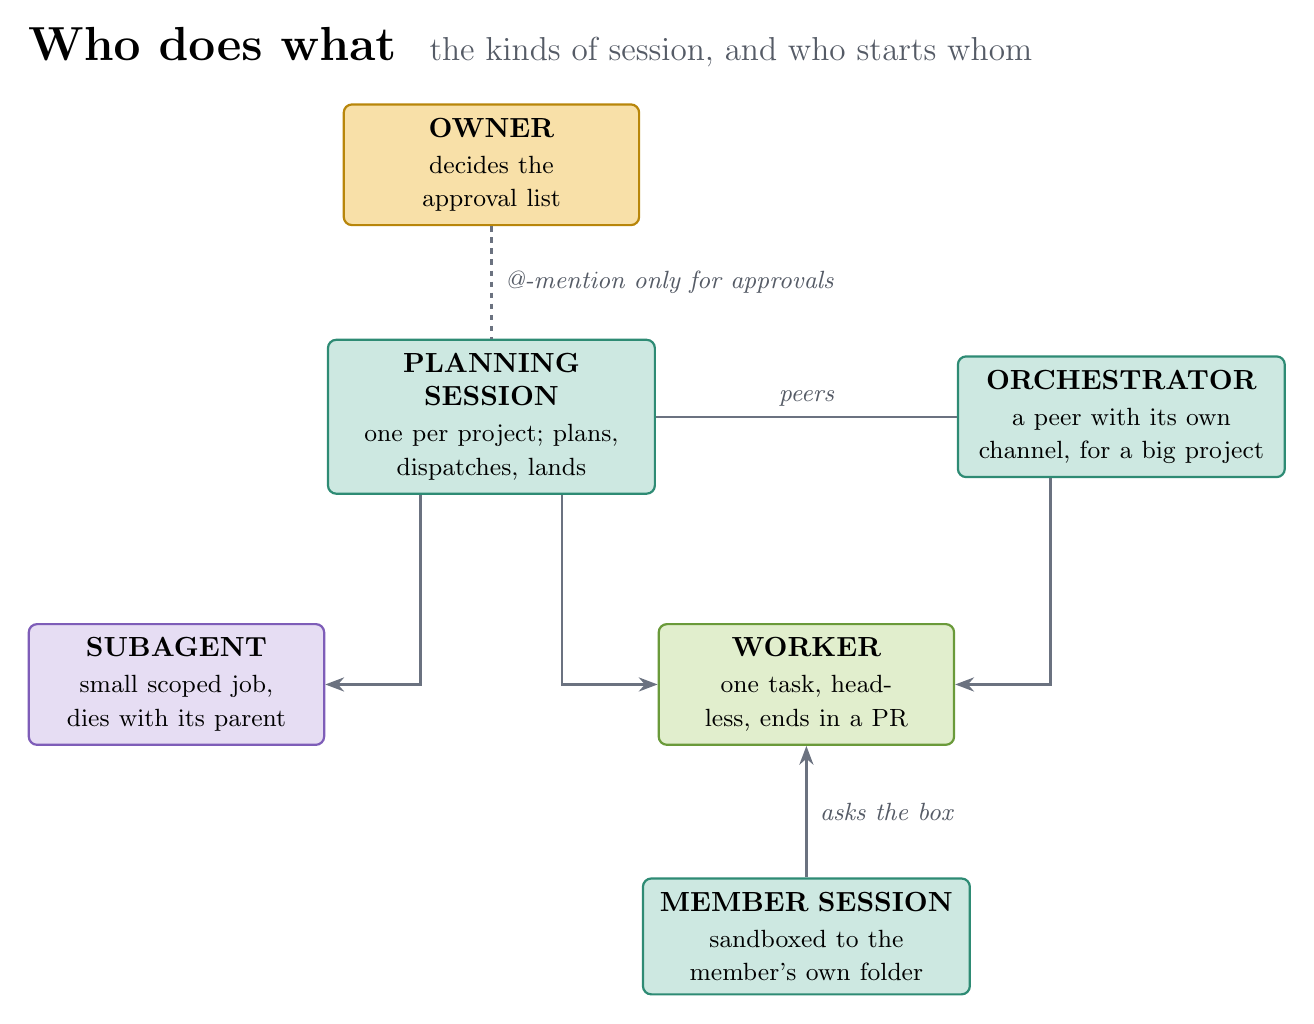
\begin{tikzpicture}
\node[person] (owner) at (0,3.2) {\nd{OWNER}{decides the approval list}};
\node[sess, text width=3.8cm] (plan) at (0,0) {\nd{PLANNING SESSION}{one per project; plans, dispatches, lands}};
\node[sess, text width=3.8cm] (orch) at (8,0) {\nd{ORCHESTRATOR}{a peer with its own channel, for a big project}};
\node[work] (worker) at (4,-3.4) {\nd{WORKER}{one task, headless, ends in a PR}};
\node[sub] (sub) at (-4,-3.4) {\nd{SUBAGENT}{small scoped job, dies with its parent}};
\node[sess, text width=3.8cm] (ms) at (4,-6.6) {\nd{MEMBER SESSION}{sandboxed to the member's own folder}};
\draw[arrC, line width=0.8pt, dash pattern=on 2pt off 2pt] (owner) -- node[lab, right=3pt, fill=none] {@-mention only for approvals} (plan);
\draw[arrC, line width=0.8pt] (plan) -- node[lab, above=2pt] {peers} (orch);
\draw[arr] ($(plan.south)+(0.9,0)$) |- (worker.west);
\draw[arr] ($(plan.south)+(-0.9,0)$) |- (sub.east);
\draw[arr] ($(orch.south)+(-0.9,0)$) |- (worker.east);
\draw[arr] (ms) -- node[lab, right=3pt] {asks the box} (worker);
\titled{Who does what}{the kinds of session, and who starts whom}
\end{tikzpicture}
\end{document}
